%\documentclass{article}
\documentclass[a4paper,12pt]{article}
% Seitenränder in schön für Steven
\usepackage[paper=a4paper,left=25mm,right=25mm,top=25mm,bottom=25mm]{geometry}
\usepackage{enumitem}
\usepackage{amsmath}
\usepackage{float}
\usepackage{graphicx}
\usepackage{tikz}
\usepackage{titling}
\usepackage{setspace}
\usepackage{amssymb}
\usepackage{caption}


\captionsetup{justification   = raggedright,
	singlelinecheck = false}

% Schusterjungen und Hurenkinder bestrafen
\clubpenalty50000
\widowpenalty50000
\displaywidowpenalty=50000

% Buchstaben mit kringel drum: %
\newcommand*\mycirc[1]{%
	\begin{tikzpicture}[baseline=(C.base)]
	\node[draw,circle,inner sep=1pt](C) {#1};
	\end{tikzpicture}}

\renewcommand{\figurename}{Abbildung}
\renewcommand{\tablename}{Tabelle}


\author{Athur 1, Author 1}
\setlength{\droptitle}{-5em} % set the title to the top of the page

% ==========================
% ===== START HERE!! =======
% ==========================
\setcounter{section}{1337} % Nummer des Aufgabenblattes
\title{ \textbf{L\"osungsblatt \thesection}}

\begin{document}	 
	\maketitle	 %Some Vodoo-magic
	
	\subsection{Erster Aufgabentitel}
	\textbf{Aufgabe/ Fragestellung}
	
	\begin{itemize}
		\item Stichpunkt 1
		\item Stichpunkt 2
		\item Stichpunkt 3
	\end{itemize}
	
	\subsection{Zweite Aufgaben\"uberschrift}
	\textbf{eine l\"angere Textaufgabe?}\\
	\\
	\textit{$comming~ soon^{_{TM}}$}
	\\
	\par
	\textcolor{red}{korrigierte Lösung in der \"Ubung mitschreiben}

	
	
	\subsection{Praktische Aufgabe}
	\textbf{Zeig uns eine coole Grafik!}
	
	\begin{figure}[h!]
		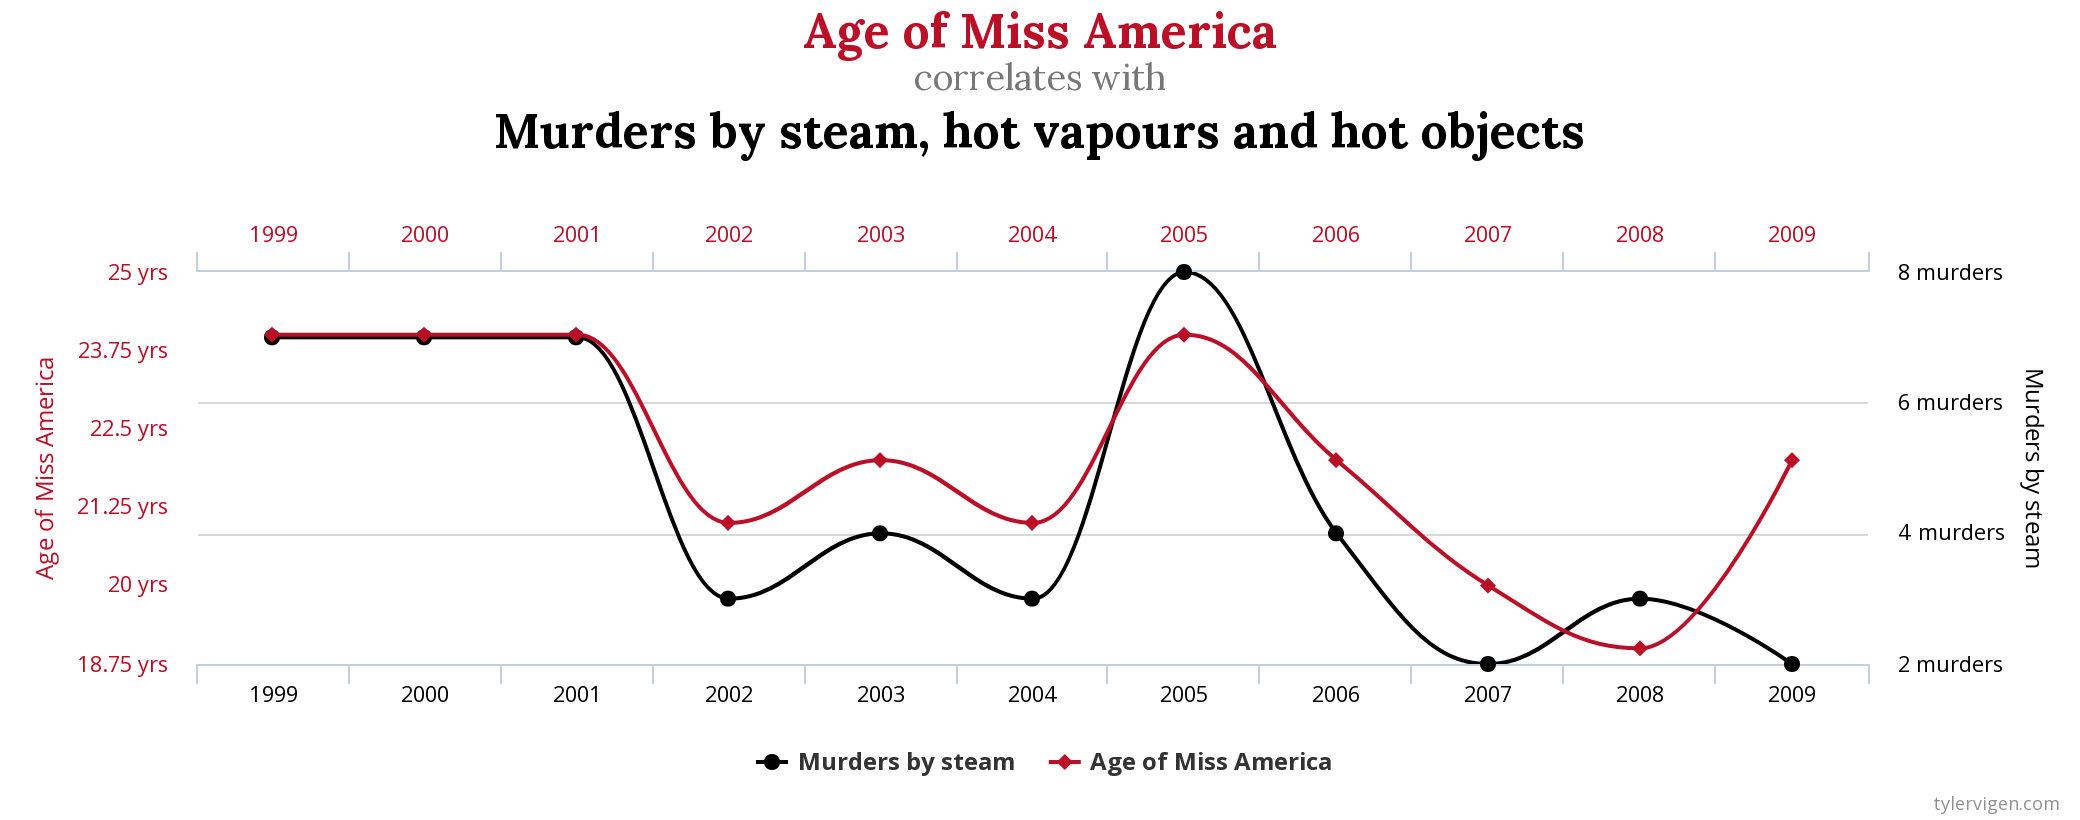
\includegraphics[width=0.85\linewidth]{chart.png}
		\caption{Bildunterschrift}
	\end{figure}
	
	
	\subsection{F\"ullt die Tabelle aus!}
	\textbf{Alles klar, chef?}
	
	\begin{table}[h!]
		\caption{quote useless table}
		\begin{tabular}{c|c|c|l}\hline
			Zeile & einsen und nullen & was anderes & Erkenntnis \\ \hline
			1 & 0111 0110 0010 & 1337 & nein \\
			2 & 0101 0010 1001 & 4207 & nein \\
			3 & 1111 0110 1100 & 1769 & nein\\ \hline
			\multicolumn{4}{c}{Man kann auch mal mehrere spalten zu einer umformen}  \\ \hline
			2. & 0101 0010 \textcolor{orange}{0000} & \textcolor{green}{>9000} & \textbf{YES!} \\
			2. & 0101 0010 0100 & 404 & nope
		\end{tabular}
	\end{table} 
	
	
	

\end{document}

% Hier nach passiert nichts mehr, daher nutzen wir das als kleines Cheat-Sheet ;)
% ===============================================================================

% Aufzählungen (auch merhstufig):
\begin{itemize}[itemsep=0pt]
	\item 
\end{itemize}

%Bilder eifnügen:
\begin{figure}[h!] %h! sorgt dafür dass das Bild möglichst nicht woanders hingeschoben wird
	%Erklärung: [width=0.5\linewidth] -> Bild ist maximal so breit wie die Hälfte des Schriftbildes
	\includegraphics[width=0.5\linewidth]{Bildname.jpg} 
	\caption{Bildunterschrift}
\end{figure}

%Tabelle einfügen:
\begin{table}[h!] %h! sorgt dafür dass die Tabelle möglichst nicht woanders hingeschoben wird
	\caption{Tabellenüberschrift}
	%hinter {tabular}: Anzahl Spalten (c=center, l=linksbündig, r=rechtsbündig, | Spaltenstriche)
	\begin{tabular}{|c|c|c} 
		A & B & C  \\ % \\ = return (neue zeile)
		\hline % horinzontale Linie
		0 & 1 & 2
	\end{tabular}
\end{table}
